\chapterpicture{header_10}
\chapter{Farmaci oppioidi}
\markboth{Farmaci oppioidi}{\printitle}

Gli oppioidi sono dei farmaci utilizzati sempre per la terapia del
dolore. A differenza dei FANS, però sono farmaci che trattano il dolore
derivante da patologie più serie rispetto all'infiammazione. Il dolore,
in questo caso, è più forte.

Il dolore cronico deriva da altre patologie, che causa anche il dolore.
Non si può agire sulla patologia in modo diretto, però è necessario
agire sul dolore.

\fullpicture*{18_001}{Soglia del dolore}

Il dolore deriva dai recettori periferici, che trasmettono un segnale al
SNC e che viene elaborato dal cervello come sensazione di dolore. La
sensazione del dolore può essere diminuita, aumentando la soglia del
dolore, in modo tale da non provarlo più.

I farmaci oppioidi danno dipendenza; questo ha causato delle situazioni
disastrose in Italia, negli anni '90. Questo perché i farmaci oppioidi
possono venire usati in modo ricreativo, con delle ripercussioni
gravissime a livello di tolleranza e di dipendenza, sia fisica che
psicologica.

Per la sintomatologia media, sono presenti degli oppioidi minori, che
possono essere associati ad antinfiammatori. Nei casi più gravi, vengono
usati gli analgesici oppioidi.

Questa classe di farmaci ha come capostipite la morfina.

A differenza dei FANS, questi farmaci agiscono a livello del sistema
nervoso centrale. Questi farmaci riescono a modulare la sensazione del
dolore, quindi aumentano la soglia del dolore.

Questi farmaci sono agonisti per certi recettori; più il recettore ha
attività, maggiore è la soglia del dolore. Questo effetto può essere
visto anche al contrario, ovvero come diminuzione della consapevolezza
del dolore.

Gli effetti collaterali di questi farmaci sono gravissimi. Innanzitutto,
inducono dipendenza, sia psicologica sia fisica. La dipendenza
psicologica è dovuta al fatto che l'attivazione di questi recettori,
detti \emph{oppioidi} comporta anche una sensazione di
euforia\ft{Il consumatore iterativo di queste molecole ricerca la sensazione dell'euforia. Però non si rende conto che questa sensazione è affiancata a dei segnali depressivi del sistema respiratorio potentissimi.}.
Un effetto collaterale è appunto la depressione respiratoria.

Oltre alla dipendenza psicologica, c'è anche una dipendenza fisica molto
grave, in quando, andando ad aumentare la soglia del dolore, si prova
meno dolore in generale. Nel momento in cui si toglie il farmaco, il
dolore provato è molto intenso. La sensazione di dolore fisico aumenta.

Questa tipologia di effetti collaterali è presente anche se si usano
queste molecole dal punto di vista terapeutico. La somministrazione e la
fine della terapia sono seguite dai medici. Non si può smettere da un
giorno all'altro di assumere questi farmaci.

Questi farmaci creano una tolleranza, quindi è necessario aumentare
sempre il dosaggio di farmaco.

\paragraph{Morfina}

La morfina è una sostanza conosciuta fin dall'antichità. Il nome
\emph{morfina} deriva da Morfeo, in quanto, inizialmente, un effetto che
gli oppiacei danno è la sedazione.

\marginpicture*{18_002}{Morfina}

Nell'antichità, si assumeva la morfina come \emph{oppio}, che deriva
dalla parola greca ``succo''. Utilizzando questo succo, si aveva un
effetto sedativo e analgesico. In seguito, con lo sviluppo della
scienza, si è studiata la composizione dell'oppio, che contiene circa 40
alcaloidi. La morfina è la sostanza più presente nell'oppio. La morfina
è stata poi isolata dall'oppio, all'inizio del
1800\ft{La morfina veniva somministrata ai feriti della guerra di secessione americana, per alleviare il dolore. Però la maggior parte di questi feriti è morta per depressione respiratoria.}.
La morfina, in seguito, è stata preparata per estrazione in larga scala.

Per determinare la struttura della molecola, si rompeva la molecola per
via chimica e si vedeva se i frammenti avevano attività farmacologica.

Solo nel 1925 si è arrivati a comprendere la struttura della morfina.
Dalla struttura, si è arrivati alla sintesi completa, nel 1952. La
struttura cristallografica è stata ottenuta nel 1964.

Dal punto di vista farmaceutico e dello sviluppo del farmaco, la storia
della morfina è affascinante; è un bellissimo esempio di sviluppo del
farmaco, a partire da una molecola naturale. Si è cercato di avere delle
relazioni struttura-attività per avere l'attività desiderata, e per
avere una molecola più facile da sintetizzare che avvia la stessa
attività.

Nel caso della morfina, visti gli effetti collaterali importanti, si
desiderava anche avere delle molecole prive di questi effetti.

\paragraph{Peptidi oppioidi}
Dopo aver identificato la struttura, ci sono state identificate dei
peptidi oppioidi endogeni, negli anni '70. Questi peptidi sono stati
isolati dal cervello; per questo si chiamano \emph{cefaline}.

Questi piccoli peptidi sono chiamati \emph{peptidi oppioidi} perché sono
agonisti dei recettori oppioidi, quindi inducono, in modo fisiologico e
funzionale, l'effetto della morfina. Queste molecole sono divise in
quattro famiglie, sulla base di analogie strutturali e funzionali:

\begin{itemize}
\item
  Encefaline
\item
  Endorfine
\item
  Dinorfine
\item
  Endomorfine
\end{itemize}

Queste sostanze vengono liberate quando si fa sport o quando si mangia
del cioccolato. Queste sostanze sono fisiologiche, quindi non porta a
nessun effetto collaterale, ma agiscono sulla stessa catena di reazioni
degli analgesici oppioidi.peptidi oppioidi

Questi peptidi si originano da alcuni precursori, in seguito al taglio
della catena peptidica. Tutti i peptidi presentano una Tyr nella parte
N-terminale.

Questi piccoli peptidi hanno una distribuzione anatomica diversa:

\begin{itemize}
\item
  Le \beta-endorfine sono presenti nel SNC e nel SNP
\item
  Le encefaline sono diffuse in tutto l'organismo
\item
  Le dinorfine sono diffuse nel SNC
\end{itemize}

\section{Recettori oppioidi}

I recettori oppioidi sono caratterizzati in tre famiglie; ogni recettore
determina degli effetti molto diversi. Essi sono

\begin{itemize}
\item
  \emph{Recettori \mu:} i recettori \mu{} sono responsabili dell'effetto
  analgesico e sedativo, ma sono anche responsabili della depressione
  respiratoria, dell'euforia e della dipendenza. La morfina lega
  fortemente con questo recettore.
\item
  \emph{Recettori \kappa:} i recettori \kappa, quando vengono legati,
  hanno un lieve effetto analgesico e sedativo, ma non hanno effetti
  sulla respirazione, non sono euforizzanti e creano poca dipendenza. La
  morfina lega meno fortemente con questo recettore.
\item
  \emph{Recettori \delta:} i recettori \delta, se sono legati, producono
  un lieve effetto analgesico, ma non producono altri effetti. La
  morfina lega meno fortemente con questo recettore.
\end{itemize}

Questi recettori sono simili tra di loro e sono accoppiati alla proteina
G, che è una proteina transmembrana.

I recettori \kappa, come nel caso delle COX-2, sono stati ricercati per
avere dei farmaci selettivi, che quindi mantengono l'effetto sedativo,
senza avere dei grossi effetti collaterali. In realtà, questi farmaci
presentano altri effetti collaterali importanti, come psicosi e
depressione. Questa strada di sviluppo del farmaco è stata abbandonata.

I recettori \mu{} hanno i seguenti effetti:

\begin{itemize}
\item
  Analgesia, a livello soprattutto cerebrale, ma anche spinale e
  periferico
\item
  Depressione respiratoria
\item
  Miosi
\item
  Effetti inibitori sul sistema cardiovascolare
\item
  Emesi
\item
  Contrazione della muscolatura liscia
\item
  Effetto anti tosse
\item
  Effetti endocrini
\item
  Immunosoppressione
\item
  Sedazione
\end{itemize}

I recettori \kappa{} invece sono mediatori di:

\begin{itemize}
\item
  Analgesia, soprattutto a livello spinale
\item
  Contrazione della muscolatura liscia
\item
  Effetti endocrini
\item
  Stimolazione del sistema cardiovascolare
\end{itemize}

Infine, i recettori \delta{} sono mediatori di:

\begin{itemize}
\item
  Analgesia a livello cerebrale e spinale
\item
  Effetti sulla funzione immune
\item
  Contrazione della muscolatura liscia
\end{itemize}

A livello farmaceutico, i recettori oppioidi \mu{} sono quelli
interessanti.
I recettori oppioidi sono simili tra di loro. Sono accoppiati alla
proteina G. Sono formati da sette eliche che si posizionano
transmembrana.

\fullpicture*{18_003}{Meccanismo di reazione dei recettori oppioidi}

L'agonista oppioide lega il recettore all'esterno e causa il segnale
legato alla proteina G, con i segnali relativi.

La proteina G attivata è detta ``inibitoria''; il secondo messaggero,
ovvero l'cAMP, rilasciato diminuisce. La diminuzione di cAMP determina
altri tre passaggi biochimici, ovvero l'apertura dei canali \ce{K+}, la
chiusura dei canali \ce{Ca^{2+}} e l'inibizione del rilascio dei
neurotrasmettitori.

Questo comporta che vengono inibiti i segnali percepiti come dolore; in
questo modo, si innalza la soglia del dolore.

I recettori oppioidi si trovano all'interno dell'SNC, dove causano degli
effetti collaterali, quali tolleranza, assuefazione, dipendenza e
sonnolenza. I recettori oppioidi si trovano anche in altre regioni
periferiche, come dell'apparato gastrico e nell'apparato intestinale.
Questo comporta altri effetti collaterali, in quanto vanno ad inibire
l'attività gastrica, causando costipazione. Questo non è un effetto
collaterale grave, però per i pazienti debilitati, può essere un
problema.

\fullpicture*{18_004}{I recettori oppioidi sono presenti anche nell'apparato intestinale}

Alcuni oppioidi vengono usati anche per aiutare la sedazione, in caso di
anestesia. L'effetto collaterale di depressione respiratoria può essere
usato a vantaggio, se vengono usati su pazienti intubati, che quindi
respirano in modo artificiale. Per rendere più efficiente l'utilizzo dei
macchinari esterni, può essere necessario indurre la depressione del
sistema respiratorio.

Ci sono altri derivati oppioidi, come la codeina, l'idrocodone e
l'idromorfone, che invece vengono utilizzati in formulazioni orali come
antitussivi, in quanto i recettori \mu{} sono collegati ai centri della
tosse.

Altri derivati, in particolare il metadone, vengono usati per trattare i
sintomi da dipendenza nei tossicodipendenti.

Dalla morfina, che è il capostipite di questa famiglia, sono state fatte
delle modifiche strutturali per aumentare o variare la via di
somministrazione, però anche gli altri oppioidi presentano tolleranza e
dipendenza fisica.

\marginbox{Tolleranza}{
Con la somministrazione frequente e ripetuta di dosi terapeutiche di morfina e analoghi, si osserva una progressiva perdita dell’effetto terapeutico.
Per riprodurre la risposta iniziale è necessario aumentare la dose.
}

\marginbox{Dipendenza fisica}{
Quando si termina la somministrazione del farmaco o si somministra un antagonista, avviene una crisi di astinenza. Per questo l’uso di oppioidi deve essere seguito da un medico.
}

Lo sviluppo di analgesici oppioidi è un esempio farmaceutico dello
sviluppo del farmaco. La chimica farmaceutica ha sfruttato le sostanze
naturali, per sviluppare dei farmaci migliori, per ridurre gli effetti
collaterali o per migliorare la potenza, in modo da utilizzare delle
dosi minori.

\paragraph{Oppio}

\marginpicture*{18_005}{Pianta di \emph{Papaver Somniferum}}

La morfina deriva dall'oppio, che viene prodotto dal \emph{Papaver
Somniferum}. La pianta trasuda un latte, che viene raccolto, fatto
seccare e assunto come stupefacente.

Il succo contiene numerosi alcaloidi, il cui principale è la morfina
(4--21\%), ma sono presenti anche la codeina (0.8--2.5\%). I vari
alcaloidi\ft{Gli alcaloidi sono delle sostanze contenenti degli atomi di azoto, che rendono le molecole alcaline.}
sono presenti in percentuali differenti, a seconda della pianta e da
dove viene coltivata.

È necessario distinguere:

\begin{itemize}
\item
  \emph{Oppiacei:} sono le sostanze naturali che si trovano all'interno
  della pianta di \emph{Papaver Somniferum}
\item
  \emph{Oppioidi:} sono sostanze che comprendono sia gli oppiacei, sia
  le sostanze di sintesi, che hanno degli effetti analgesici. Le
  endorfine e le altre sostanze endogene sono dette \emph{oppioidi
  endogeni}.
\end{itemize}

\section{Morfina}

La struttura della morfina è una struttura molto particolare, con delle
caratteristiche strutturali, farmacodinamiche e farmacocinetiche
interessanti.

\marginpicture*{18_006}{
Morfina. Il nome IUPAC è
\emph{(5\alpha,6\alpha)-7,8-dideidro-4,5-epossi-17-metilmorfinan-3,6-diolo}
indica la presenza di un epossido, però in realtà è presente un anello a
cinque termini, quindi è assimilabile a in furano parzialmente
idrogenato. Questo errore è presente anche negli altri derivati
oppioidi.}

Si possono identificare vari aspetti strutturali caratteristici, come la
struttura molto rigida, che permette di bloccare i gruppi interagenti
con il recettore.
Nella posizione 3 e 6 sono presenti due gruppi ossidrili. L'ossidrile in
3 è fenolico, e quindi sarà più acido rispetto all'altro ossidrile.
Questo lo rende un buon donatore di legame a idrogeno.
Il doppio legame presente in posizione 7 e 8 rende l'ossidrile presente
in posizione 6, un alcol allilico, che sicuramente partecipa come
donatore di legame ad idrogeno.
Il sistema aromatico dona una importante funzionalità per l'interazione
con il recettore.

La molecola è formata da quattro anelli, a cui se ne aggiunge un quinto,
che è formato da un ponte ossigeno.
Sono presenti molti centri chirali e la stereochimica è molto precisa.
La struttura attiva è quella mostrata in figura; se si cambia un solo
centro stereochimico, l'attività viene persa o molto diminuita.
La morfina possiede un anello piperidinico, che contiene un atomo di
azoto basico, per questo è un alcaloide. L'ammina in questione è
presente in posizione 17 ed è una ammina terziaria.

La molecola ha un core idrofobico, però possiede un shell esterno che
permette alla struttura di stare bene in acqua. I gruppi interattivi
sono bloccati all'interno di una struttura rigida; questo è importante
per mantenere il farmacoforo, ovvero lo schema interattivo con il
proprio recettore. Il \(\log{} P\) è pari a 0.8.

\marginpicture*{18_007}{Farmacoforo della morfina.}

\begin{figure}[H]
  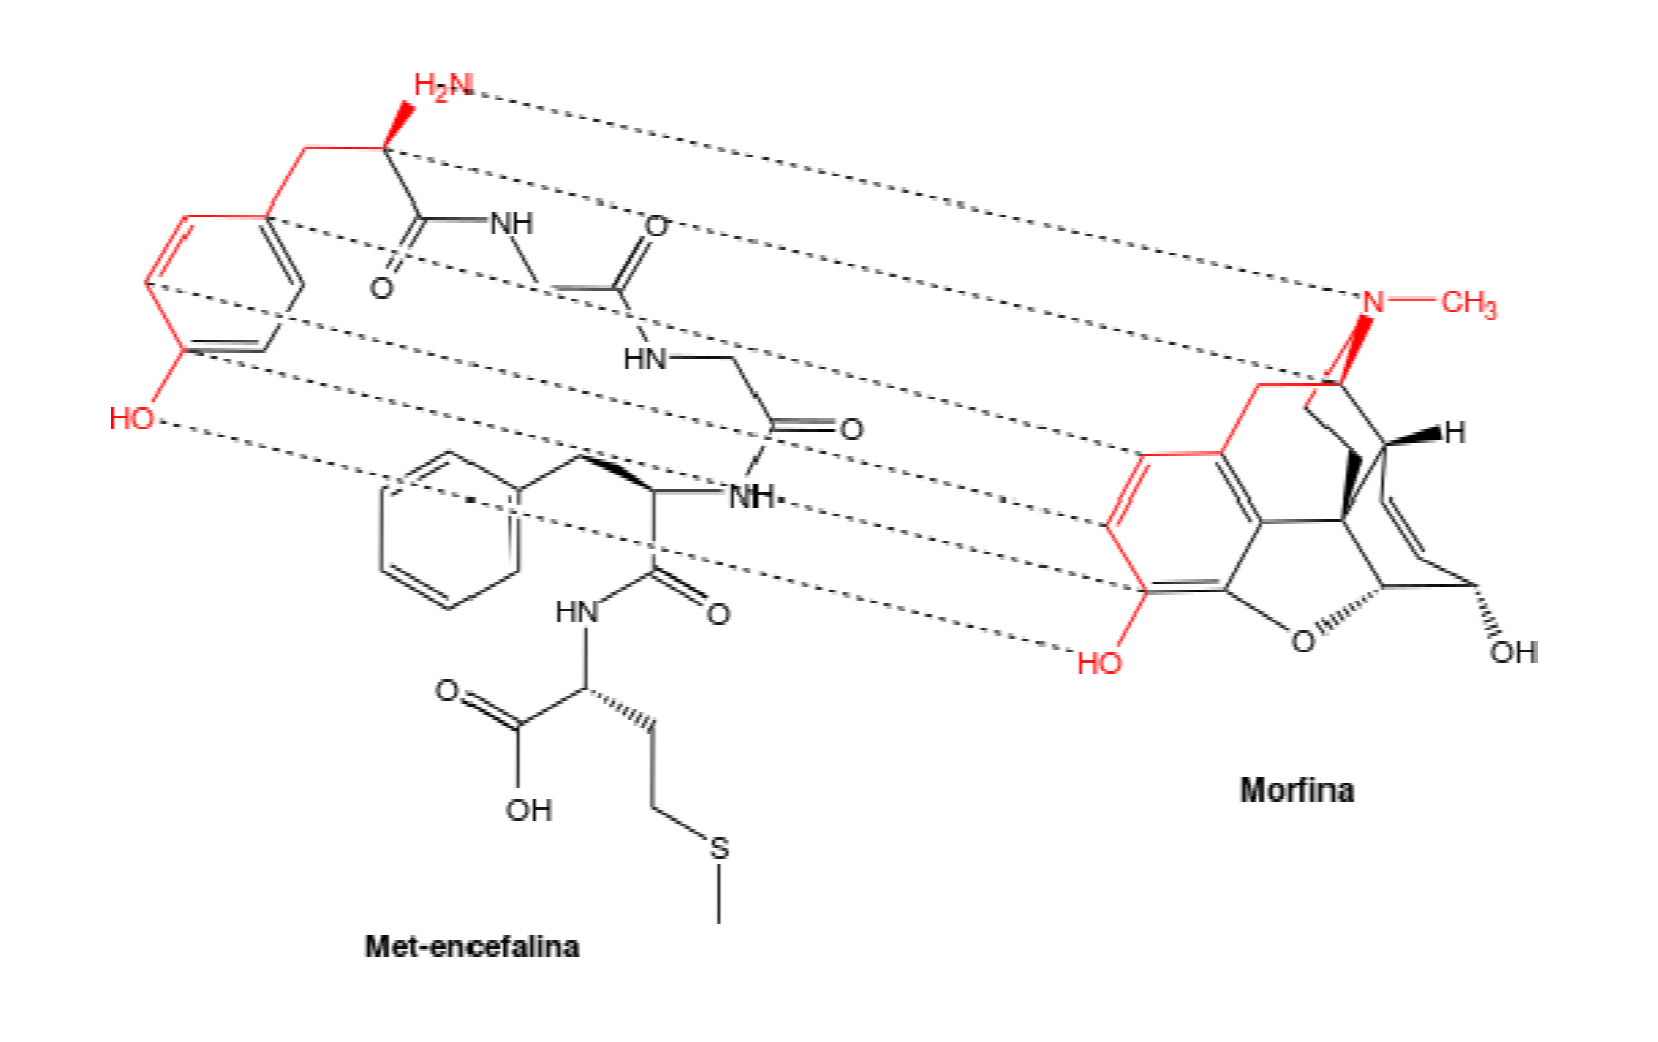
\includegraphics[width=0.8\textwidth]{18_008}
  \caption{Confronto tra gli oppioidi endogeni e la morfina. Si vede che
  la Tyr N-terminale degli oppioidi endogeni ricorda la struttura della
  morfina. Questo conferma il farmacoforo della struttura e quindi quali
  sono le funzioni importanti per avere l'effetto analgesico legato a
  queste sostanze.\\
  Entrambe le ammine sono sono protonabili, invece il gruppo ossidrilico è
  fenolico in entrambi i casi, quindi può formare legami a idrogeno
  facilmente.\\
  La struttura della morfina è bloccata, mentre nei peptidi è più libera;
  questa struttura è adatta per legare i recettori \mu.}
\end{figure}

\newpage

\fullpicture*{18_009}{L'azoto dell'anello piperidinico è essenziale per l'interazione
con il bersaglio, infatti l'analogo con il carbonio non presenta
attività. L'analogo con l'azoto quaternario non è attivo, almeno nel
SNC, in quanto non può superare la barriera ematoencefalica.}

A causa del basso \(\log{} P\), la morfina ha un problema di
biodistribuzione, in quanto deve superare la barriera ematoencefalica
per raggiungere il sistema nervoso centrale. Questa molecola non
somministrata per via orale, in quanto solo una piccola parte entra nel
SNC.

La difficoltà nell'attraversare le barriere è legata alla possibile
presenza di cariche, che rendono difficile l'attraversamento.

La morfina viene somministrata per via iniettiva, in quanto si riesce ad
eliminare l'assorbimento gastrointestinale. Una concentrazione elevata
di morfina può attraversare le membrane, raggiungendo quindi il sistema
nervoso centrale.

Esistono comunque delle formulazioni per l'assunzione orale, come il
solfato di morfina, però sono meno efficienti rispetto alla via
iniettiva. Queste formulazioni vengono usate per il trattamento di
dolori lievi.

La morfina viene metabolizzata a livello epatico, per poi essere
eliminata. Si ha la demetilazione del gruppo metile legato all'azoto; la
molecola ottenuta si chiama \emph{nor-morfina}. Un altra modifica che
avviene a livello epatico è il legame dei gruppi ossidrili con l'acido
glucuronico\ft{Si trovano nelle urine.}.
\begin{figure}[H]
  \centering
  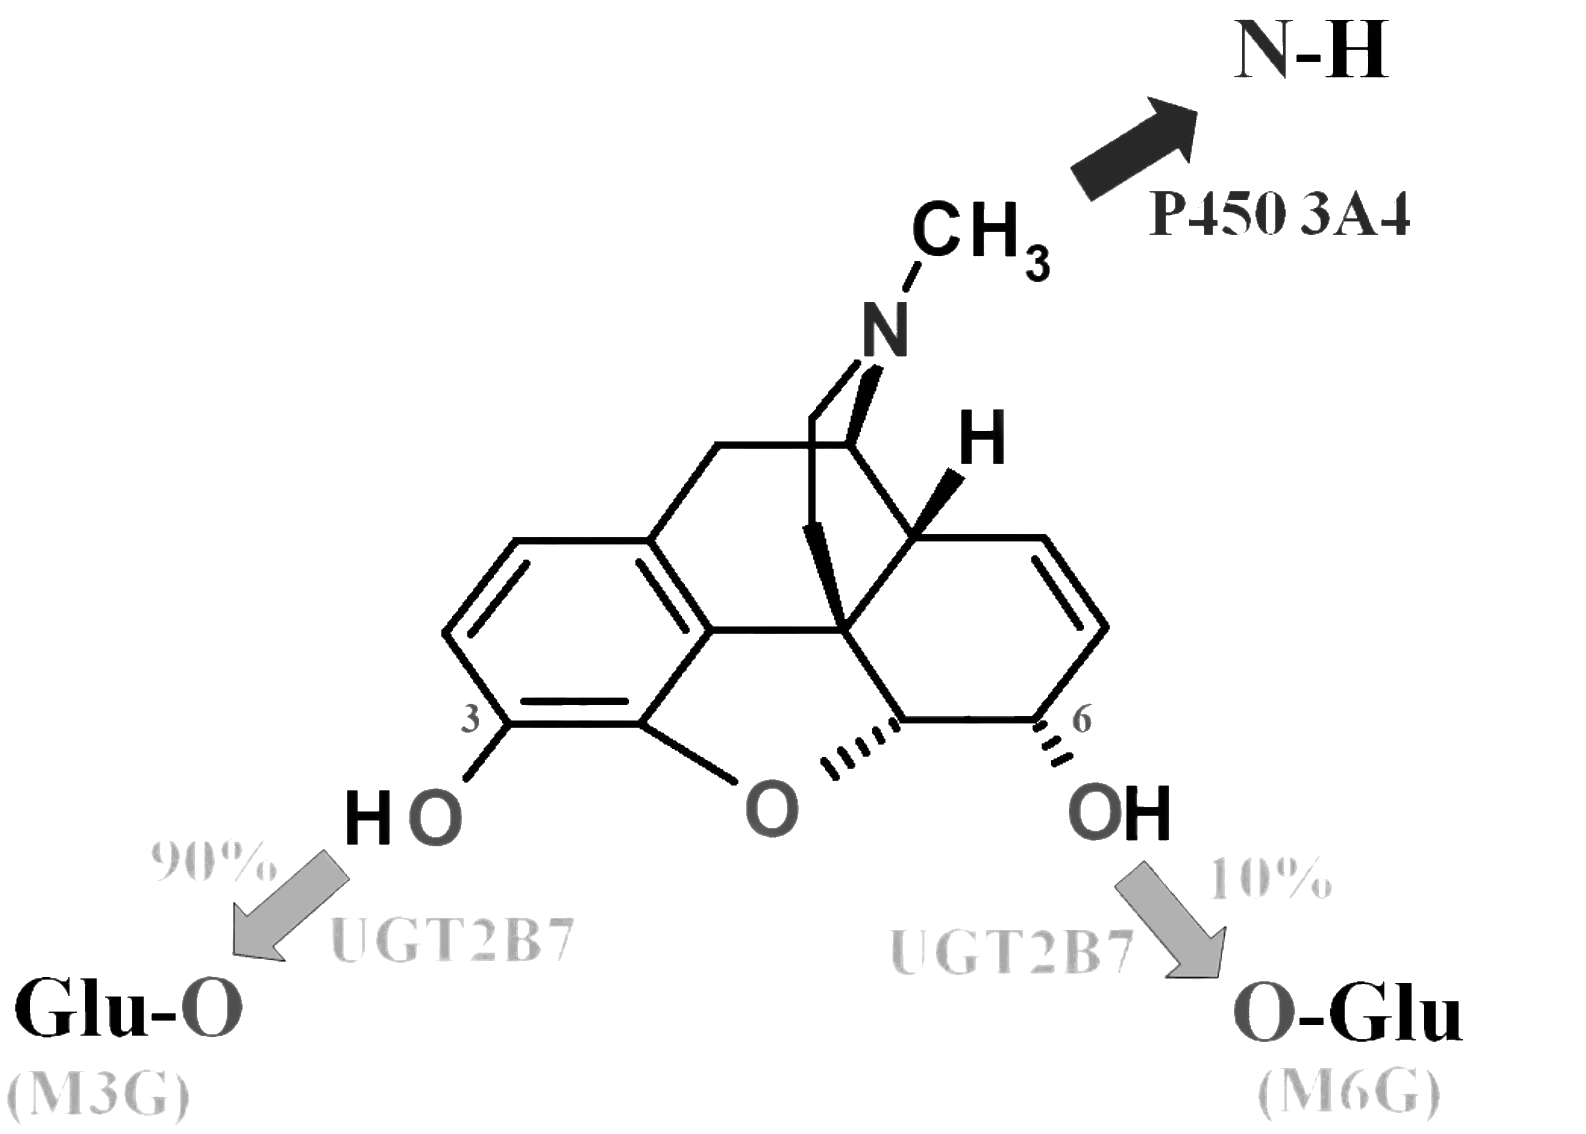
\includegraphics[width=0.6\textwidth]{18_010}
\end{figure}


Queste modifiche serviranno in seguito per migliorare la farmacocinetica
della morfina, in quanto quando la morfina arriva nel fegato, viene
metabolizzata velocemente.

La morfina è una molecola che non è farmaceuticamente ottimale, perché
ha una bassa biodistribuzione e viene metabolizzata velocemente. Ciò
determina una via di assunzione non ottimale e una bassa emivita.
Nonostante queste caratteristiche, la morfina è un buon farmaco.

\section{Codeina}

La codeina è il metil-derivato della morfina

\marginpicture*{18_011}{Codeina}

La codeina non è attiva e per questo viene definita come un pro-farmaco.
La codeina viene demetilata e diventa morfina. Questo comporta che la
codeina possa venire somministrata per via orale senza avere gli effetti
collaterali a livello gastrointestinale della morfina. Quando raggiunge
il fegato, viene demetilata e diventa attiva. Solamente il 10\% della
codeina viene convertita in morfina.

La codeina viene utilizzata come sciroppo
antitussivo\ft{La codeina può essere usata anche sui bambini, però i pediatri ne sconsigliano l'uso.}.
L'assunzione della codeina per via orale permette di avere degli effetti
collaterali molto ridotti rispetto alla morfina.

La presenza del metile alza il \(\log{} P\), che è pari a 1.2, quindi
migliora la
biodisponibilità\ft{Il $\log{} P$ ideale per superare la barriera ematoencefalica si aggira intorno a 3.}
di questo farmaco.

La codeina, oltre a diventare morfina per demetilazione in posizione 3,
può diventare anche \emph{nor-codeina} per demetilazione del gruppo
metilico legato all'azoto.
\begin{figure}[H]
  \centering
  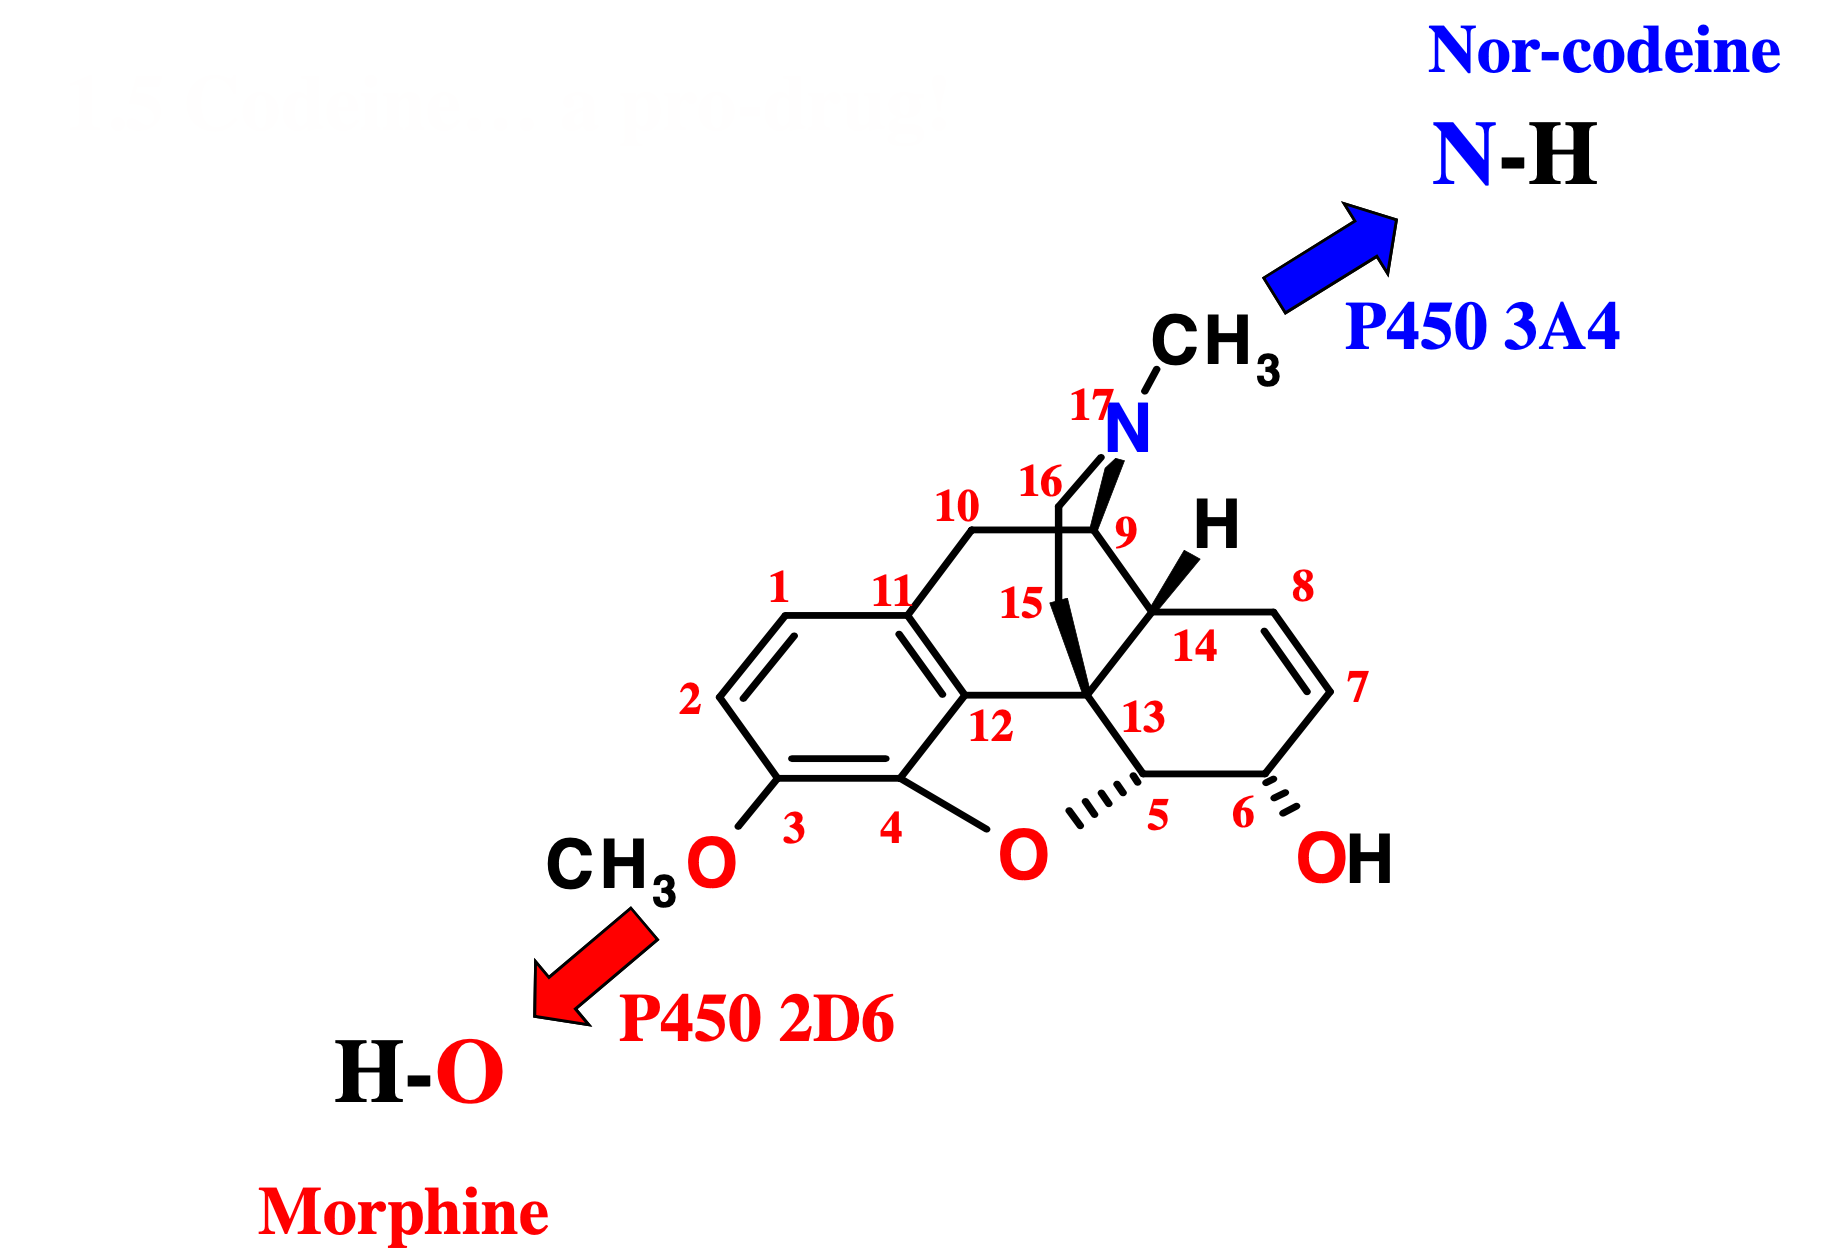
\includegraphics[width=0.8\textwidth]{18_012}
\end{figure}

L'uso di farmaci a base di codeina è sicuro, in quanto la quantità di
morfina introdotta è ridotta. Le formulazioni di codeina sono, nella
maggior parte dei casi, per via orale. L'effetto
ricreativo\ft{Vedi *purple drank* o *lean*} della codeina non è così
intenso, però è sufficiente per creare dipendenza. Tutti i farmaci, più
o meno, presentano un effetto euforizzante.

Un ulteriore utilizzo della codeina è in associazione ad altri
antinfiammatori, che consente di avere la riduzione dell'infiammazione
associata alla riduzione del dolore.

\clearpage

\section{Eroina}

Inizialmente, l'eroina è stata sviluppata come farmaco analgesico.
L'eroina in seguito è stata ritirata dal commercio ed è diventata una
sostanza stupefacente.

\marginpicture*{18_013}{Eroina}

L'effetto dell'eroina è molto diverso da quello di morfina e codeina.

L'eroina è il derivato diacetilato della morfina. L'eroina non viene
assunta per via orale, in quanto verrebbe convertita in morfina nello
stomaco e nell'intestino.

Si nota che il \(\log{} P\) è pari a 1.6, che è ancora più alto della
codeina, quindi raggiunge ancora più velocemente il sistema nervoso
centrale. L'eroina, se iniettata, raggiunge rapidamente il sistema
nervoso centrale e, solo dopo aver attraversato la barriera
ematoencefalica, viene metabolizzata in
\emph{6-monoacetilmorfina}\ft{La 6-monoacetilmorfina è un metabolita specifico dell'eroina e viene usato per identificare l'assunzione di eroina.},
che è il derivato monoacetilato in posizione 6. In seguito viene
metabolizzata a morfina.
\begin{figure}[H]
  \centering
  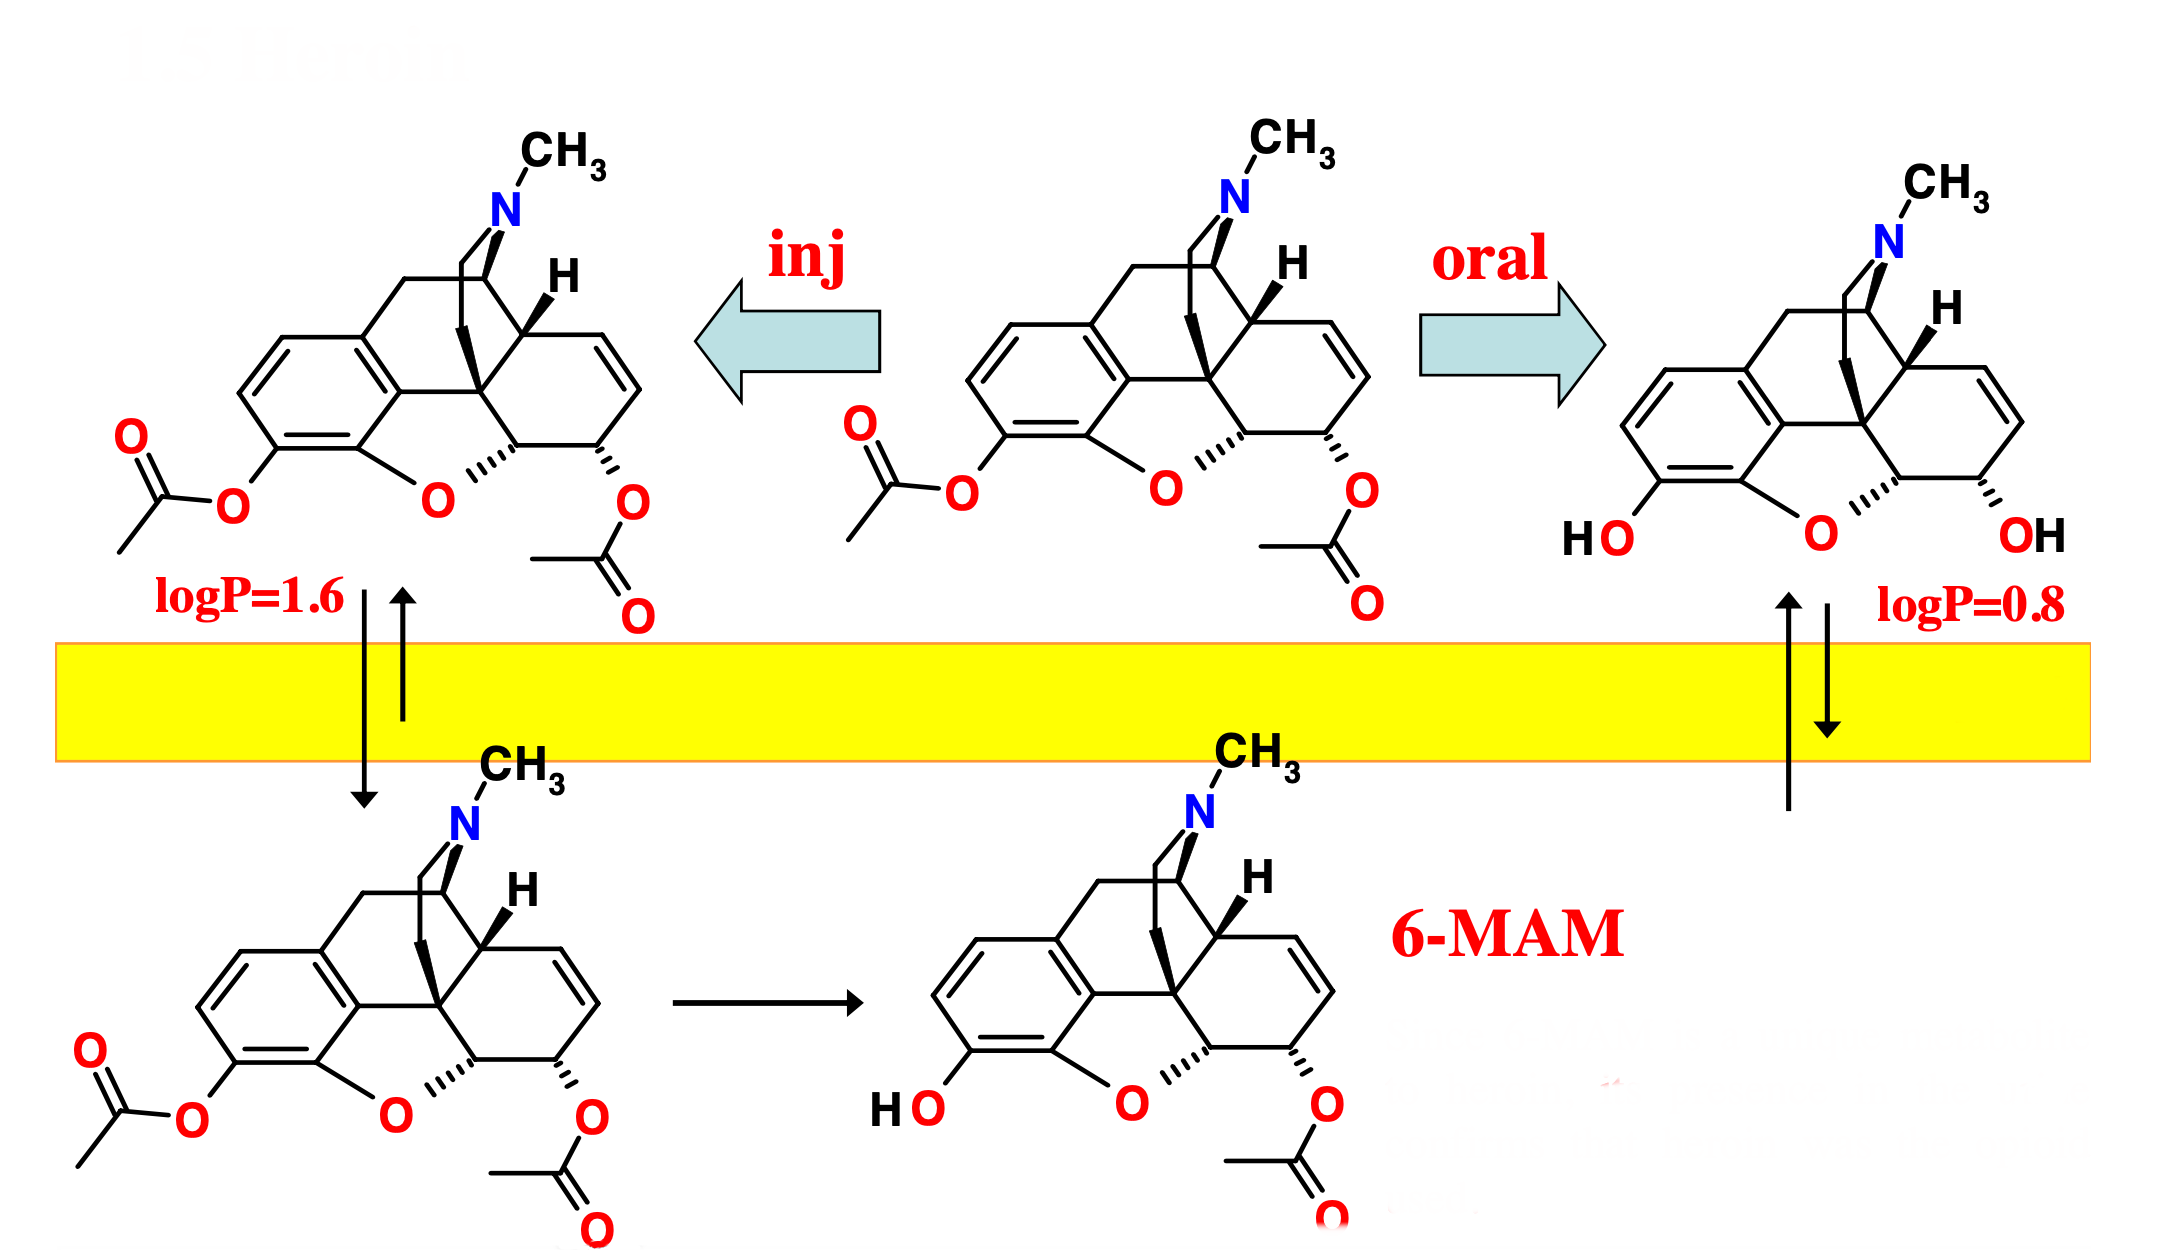
\includegraphics[width=0.8\textwidth]{18_014}
\end{figure}

La molecola attiva rimane sempre la morfina, però le modifiche
effettuate determinano una differente biodisponibilità e un diverso modo
di distribuirsi.

L'eroina non viene utilizzata in ambito terapeutico e non è considerata
un farmaco. L'eroina viene utilizzata solo in certi Stati e solo su
pazienti terminali, per ridurre il dolore e per dare una sorta di
tranquillità al paziente.

Una caratteristica dell'utilizzo di oppioidi è la \emph{miosi}, ovvero
la diminuzione del diametro della pupilla, al contrario degli
allucinogeni che causano la \emph{midriasi}, ovvero la dilatazione della
pupilla.

\section{Idromorfone e idrocodone}

\marginpicture*{18_015}{Idromorfone e idrocodone}
La morfina ha un emivita bassa, quindi sono stati sviluppati dei farmaci
che presentano un gruppo carbonile al posto del gruppo ossidrilico in
posizione 6.

Nell'idromorfone, il gruppo 6 diventa un chetone e le posizioni 7 e 8,
che prima erano legate tramite un doppio legame, sono state idrogenate.

L'idromorfone è più attivo della morfina, anche se il \(\log{} P\) resta
quasi invariato (\(\log{} P = 0.9\) ), però cambia il metabolismo; il
carbonile in posizione 6 non si lega più all'acido glucuronico, quidni
ha un emivita maggiore.

Il doppio legame deve sparire, in quanto sarebbe possibile la formazione
di un enolato, che è più reattivo rispetto ad un
chetone\ft{Quando si sostituisce un gruppo ossidrilico con un gruppo carbonilico, bisogna sempre prestare attenzione alle possibili tautomeri e/o equilibri della molecola}.

L'idrocodone, invece, è il metil-derivato dell'idromorfone, come la
codeina per la morfina. L'idrocodone ha un \(\log{} P\) pari a 1.2,
quindi può essere utilizzato anche per via orale ed è 10 volte più forte
della morfina. È noto anche come Vicodin\ft{House, M.D.}

\section{Naloxone}

\marginpicture*{18_016}{Naloxone e ossimorfone}
Fino ad ora sono stati esposti degli agonisti dei recettori oppioidi,
però esistono anche degli antagonisti. Il più comune è il
\emph{naloxone}.

Il naloxone non ha un'azione antidolorifica, in quanto non riduce la
sensazione di dolore, ma riduce la soglia di dolore. Il naloxone invece
viene utilizzato per antagonizzare gli effetti collaterali degli altri
oppioidi che portano alla morte. Commercialmente, viene chiamato
\emph{Narcan} e viene somministrato per via iniettiva. È un farmaco
salvavita e serve per contrastare un overdose da oppioidi.

Il naloxone deriva dall'ossimorfone, che rispetto all'idromorfone
possiede un gruppo ossidrile, aumentando l'attività agonista. Il
naloxone, rispetto all'ossimorfone, ha un gruppo allilico legato
all'azoto amminico. Non si sa spiegare l'attività antagonista di questo
farmaco.

\section{Oppioidi sintetici}

\fullpicture{18_017}{Riassunto relazioni struttura-attività}{fig:RiasOpi}

Nell'immagine \ref{fig:RiasOpi} è presente un riassunto delle relazioni struttura-attività
della morfina.

Dalla morfina si è cercato di semplificare la struttura, in quanto la
sintesi chimica della morfina è piuttosto complicata.

Lo schema farmacoforo è composto dai carboni 1, 2, 3, 11, 10, 16,
dall'azoto in posizione 17 e dall'ossidrile legato al carbonio 3.
Togliendo tutti i gruppi funzionali aggiuntivi, si resta con una
molecola che viene definita \emph{morfinano}, che comunque mantiene una
certa attività.
\begin{figure}[H]
  \centering
  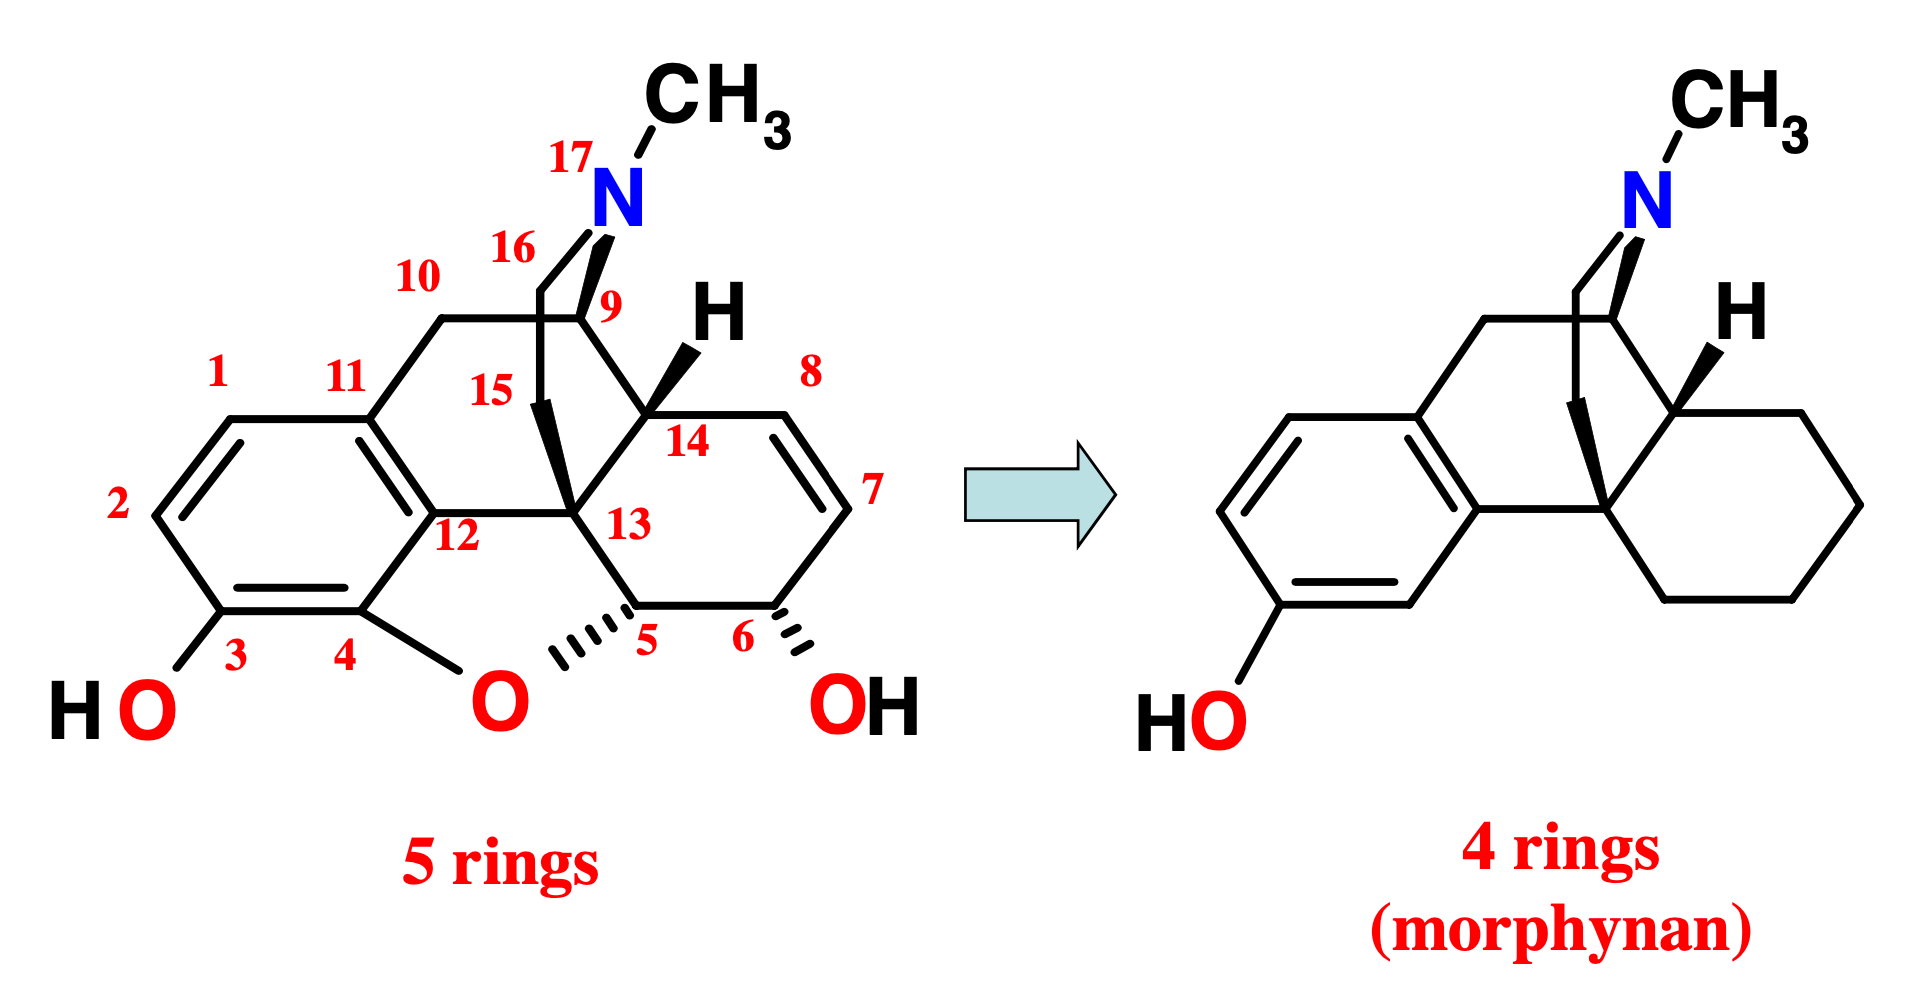
\includegraphics[width=0.6\textwidth]{18_018}
\end{figure}

\paragraph{Levorfanolo}
\marginpicture*{18_019}{Levorfanolo}
Un esponente dei morfinani è il \emph{levorfanolo}. L'attività viene
diminuita, però il \(\log{} P\) è pari a 3.1; è più alto, quindi
consente un migliore attraversamento della barriera ematoencefalica.

Si è provato anche a togliere un anello, ottenendo così i
\emph{benzomorfani}.
\begin{figure}[H]
  \centering
  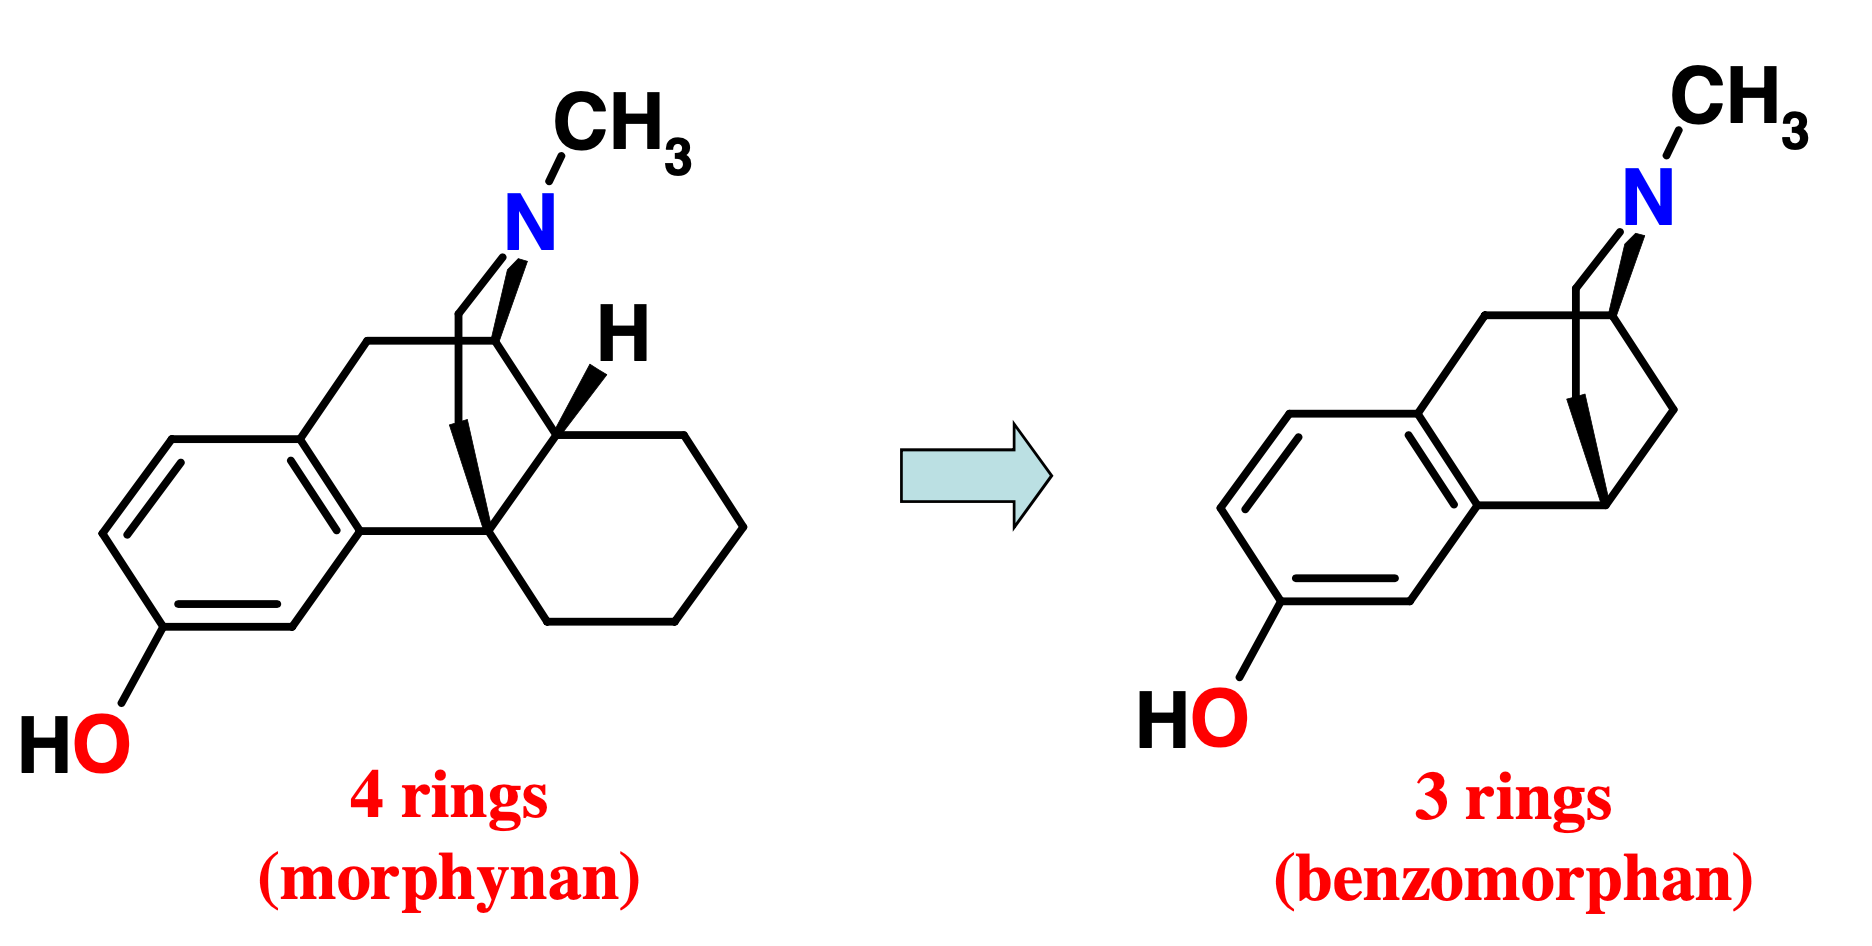
\includegraphics[width=0.6\textwidth]{18_020}
\end{figure}

\paragraph{Pentazocina}
\marginpicture*{18_021}{Pentazocina}
Un esponente dei benzomorfani è la \emph{pentazocina}, che presenta
anche il gruppo allilico, che consente alla molecola di essere un
antagonizzante dei recettori.

Questa molecola è una molecola attiva, che può essere somministrata
anche per via orale, in base alle sue caratteristiche di
\(\log{} P = 4.6\). Ha un'attività analgesica di media intensità,
proprio perché funge sia da agonista, che da antagonista, per via della
presenza del gruppo allilico.

Si è provato ancora a semplificare la struttura, eliminando un secondo
anello. Queste strutture sono definite \emph{fenilpiperidine} e
mantengono ancora una certa attività.
\begin{figure}[H]
  \centering
  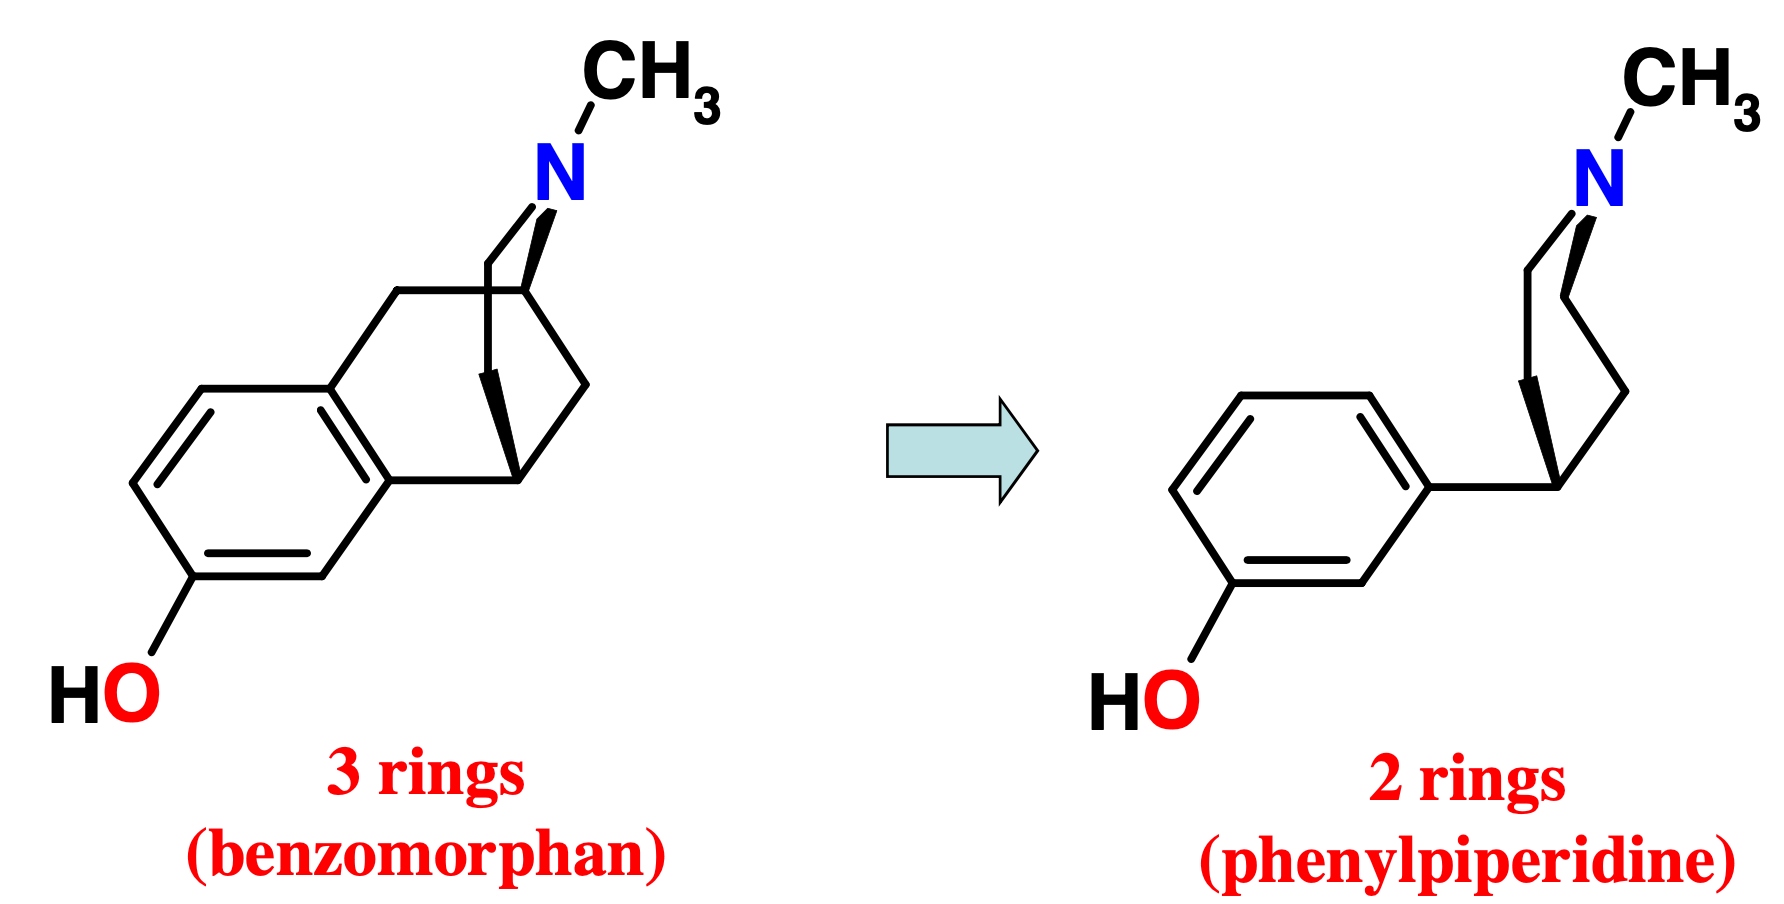
\includegraphics[width=0.6\textwidth]{18_022}
\end{figure}

\paragraph{Fentanyl}
\marginpicture*{18_023}{Fentanyl}
Da questa struttura si è partiti a fare delle modifiche bioisosteriche.
Il prodotto di queste modifiche è il \emph{fentanyl}.

Il fentanyl è un farmaco che può essere somministrato per via orale,
visto che il \(\log{} P\) è pari a 4.1. L'attività del fentanyl è 100
volte superiore a quella della morfina. Anche questa molecola è
pericolosa, più dell'eroina.

La struttura del fentanyl non ricorda esattamente quella della morfina,
però possiede lo stesso schema interattivo.

\begin{figure}[H]
  \centering
  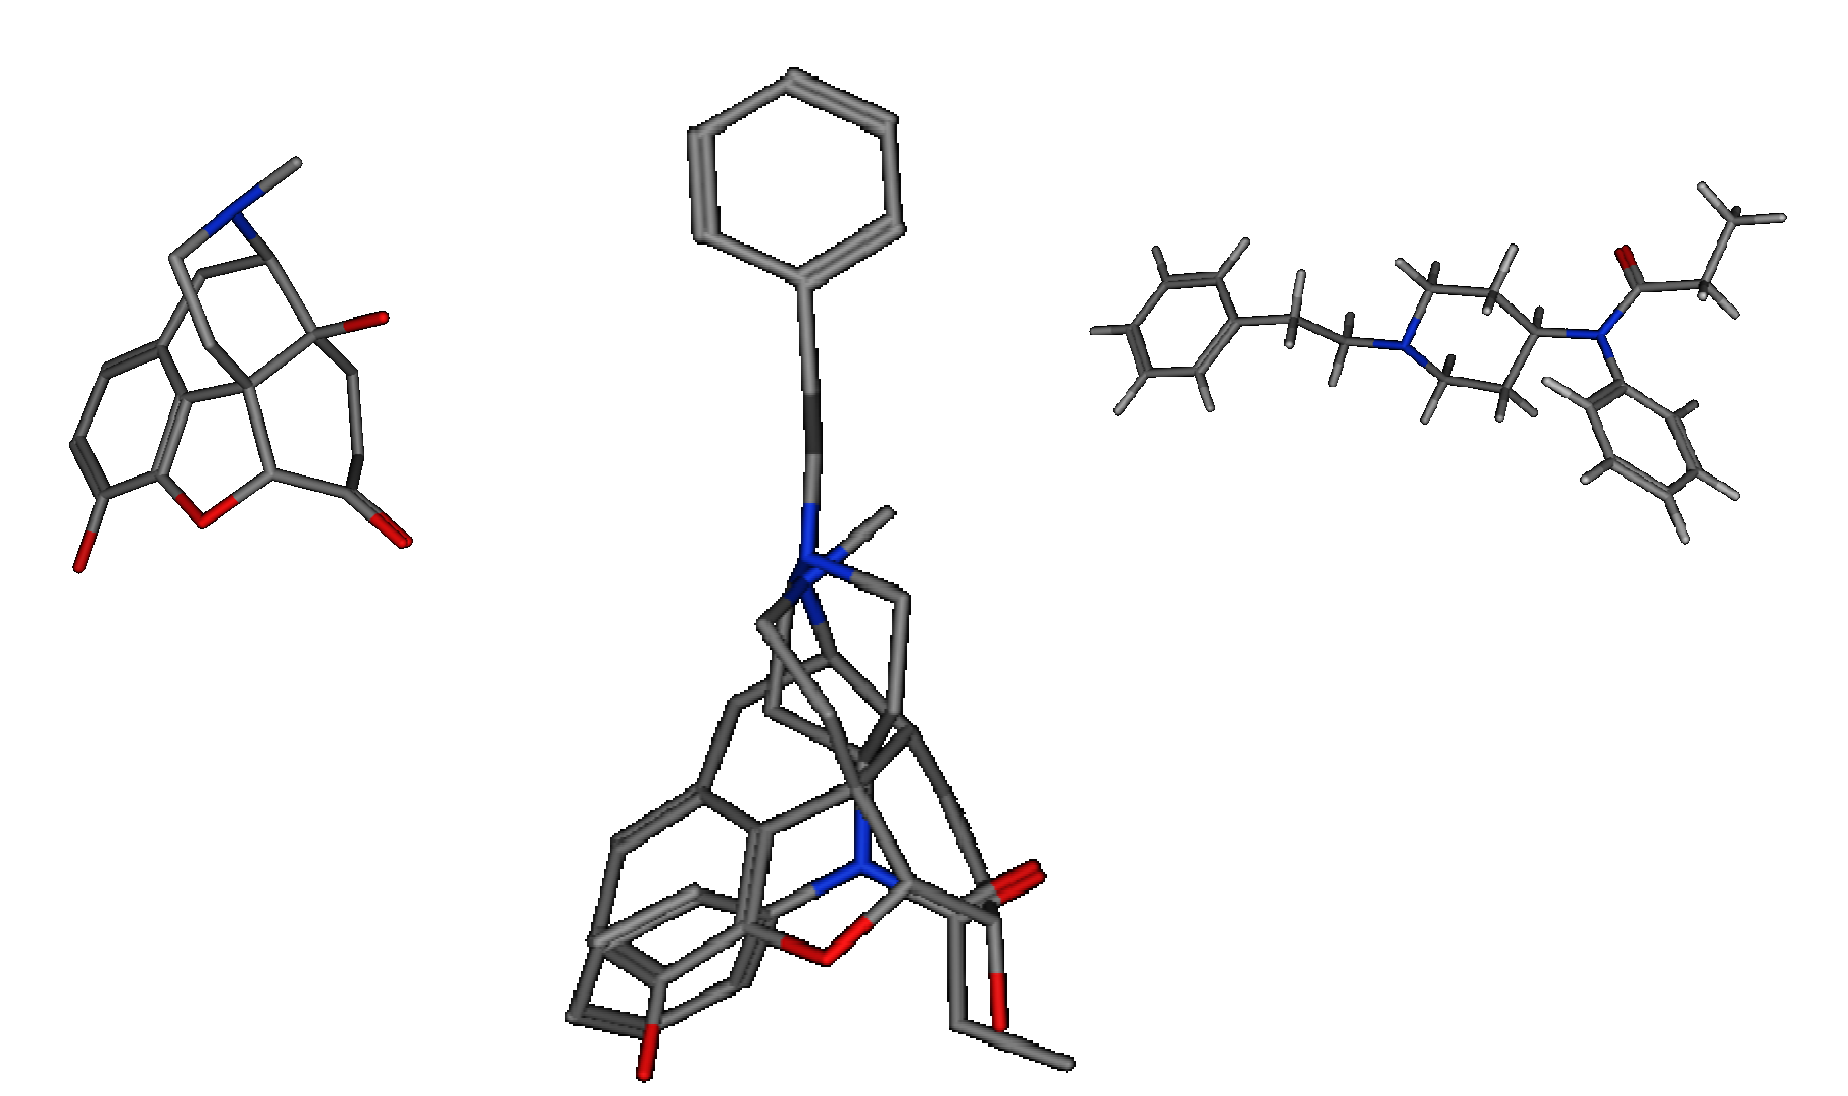
\includegraphics[width=0.8\textwidth]{18_024}
  \caption{Schema interattivo del fentanyl e della morfina}
\end{figure}

I gruppi presenti nel fentanyl sono molto diversi da quelli presenti
nella morfina. In particolare, l'azoto in posizione 17 viene sostituito
da una catena con un anello aromatico terminale, mentre l'anello
aromatico della morfina rimane intatto.

\paragraph{Loperamide}
\marginpicture*{18_025}{Loperamide}
La loperamide è contenuta all'interno di Imodium. La loperamide è una
molecola che funge da agonista per i recettori oppioidi, e quindi ha lo
schema interattivo uguale a quello della morfina.

Deve essere assunto per via orale, per raggiungere il tratto
gastrointestinale. Questo oppioide non ha effetti a livello del sistema
nervoso centrale, anche se avrebbe tutte le caratteristiche per farlo,
come il \(\log{} P\) pari a 5.5. Uno degli effetti degli oppiacei è la
costipazione.

La loperamide ha degli effetti sono a livello periferico, in quanto
esistono dei trasportatori nella barriera ematoencefalica che non
permettono il trasporto di sostanze estranee. Una volta che riconoscono
queste sostanze, le eliminano. La loperamide cerca di entrare, ma non ci
riesce.

\paragraph{Metadone}
\marginpicture*{18_026}{Metadone}
Il metadone ha tutte le caratteristiche di agonista dei recettori
oppioidi, ma viene utilizzato per le sindromi da astinenza da oppioidi,
anche a causa delle sue caratteristiche farmacocinetiche. Il
\(\log{} P\) è pari a 3.9

Il metadone comunque è attivo a livello del sistema nervoso centrale,
quindi possiede tutti gli effetti collaterali caratteristici degli altri
farmaci.

Il metadone può essere anche assunto per via orale, quindi è una misura
di controllo per il percorso di disintossicazione del tossicodipendente.